\documentclass[11pt,a4paper]{article}

\usepackage[utf8]{inputenc}
\usepackage[T1]{fontenc}
\usepackage{lmodern}
\usepackage[margin=2.2cm]{geometry}
\usepackage{booktabs}
\usepackage{tabularx}
\usepackage{array}
\usepackage{graphicx}
\usepackage{float}
\usepackage{amsmath}
\usepackage{xcolor}
\usepackage{listings}
\usepackage{fancyhdr}
\usepackage[colorlinks=true,linkcolor=blue!60!black,urlcolor=blue!60!black,citecolor=blue!60!black]{hyperref}

\definecolor{sgslate}{HTML}{0F172A}
\definecolor{sgmuted}{HTML}{475569}
\definecolor{sgcodebg}{HTML}{F8FAFC}

\lstset{
  basicstyle=\ttfamily\small,
  backgroundcolor=\color{sgcodebg},
  frame=single,
  rulecolor=\color{sgmuted!30},
  breaklines=true,
  columns=fullflexible
}

\pagestyle{fancy}
\fancyhf{}
\lhead{\small SafeGuard — Technical Report}
\rhead{\small Deep Learning \& MLOps (Axis 3)}
\cfoot{\small\thepage}
\renewcommand{\headrulewidth}{0.4pt}

\title{
  \vspace{-1cm}
  {\large \textsc{Deep Learning Avancé \& MLOps — Module Project (Axis 3)}}\\[0.4cm]
  \textbf{\Huge SafeGuard}\\[0.25cm]
  {\Large Real-Time Construction PPE Detection, Anonymous Worker Tracking, and Reproducible End-to-End MLOps Platform}
}
\author{
  \textbf{Khaled Briki} \textit{(Lead Deep Learning / Research Scientist)} \\
  \textbf{Mohamed Amine Guesmi} \textit{(Lead MLOps / DevOps Engineer)} \\
  \textbf{Oussama Ferchichi} \textit{(Lead Full-Stack Software Engineer)} \\[0.35cm]
  \small Instructor: Haythem Ghazouani \quad | \quad Academic Year: 2026--2027
}
\date{November 26, 2026}

\begin{document}
\maketitle

\begin{abstract}
\noindent SafeGuard is an end-to-end decision-support prototype for real-time Personal Protective Equipment (PPE) monitoring on construction sites (Axis 3: Real-Time Object Detection). The system combines an auditable dataset engineering pipeline (two CC BY 4.0 datasets harmonized to a 5-class canonical taxonomy with zero train/test leakage), six controlled YOLO training experiments tracked in MLflow (\texttt{EXP-A}--\texttt{EXP-F}), verified PyTorch-to-ONNX export and same-hardware runtime benchmarking, an asynchronous FastAPI inference backend backed by ONNX Runtime, a decoupled 4-stage anonymous ByteTrack + spatial PPE compliance engine, a React + TypeScript industrial operations console verified end-to-end in Google Chrome via Playwright, and containerized Docker Compose orchestration with CPU-compatible GitHub Actions CI workflows. By design, SafeGuard surfaces \emph{potential} missing-helmet events solely from explicitly learned \texttt{no\_helmet} detections requiring human review, avoids biometric re-identification, and never interprets missing positive PPE detections as proof of violation.
\end{abstract}

\tableofcontents
\newpage

\section{Introduction and Problem Statement}

\subsection{Industrial Motivation}
On active construction sites, manual verification of Personal Protective Equipment (hard hats, high-visibility vests, protective gloves) does not scale continuously across camera feeds and work zones. SafeGuard addresses real-time visual detection and structured operational alerting while adhering strictly to realistic decision-support boundaries: automated computer vision assists human safety supervisors rather than issuing autonomous disciplinary judgments.

\subsection{Architectural Principles and Constraints}
SafeGuard enforces strict decoupling between offline model engineering and online runtime serving:
\begin{enumerate}
  \item \textbf{Training vs.\ Runtime Isolation}: The FastAPI serving container (\texttt{backend/Dockerfile}) installs only ONNX Runtime, FastAPI, Pydantic, NumPy, Pillow, OpenCV-headless, and PyYAML. PyTorch, Ultralytics, DVC, MLflow, and datasets are completely excluded from runtime layers.
  \item \textbf{Canonical Taxonomy Gate}: Every data pipeline script, training YAML, ONNX metadata file, backend validator, and compliance rule resolves class IDs from a single YAML specification (\texttt{configs/class\_mapping.yaml}).
  \item \textbf{Leakage Prevention First}: Exact SHA-256 hashing, perceptual hashing (pHash), and video-stem scene grouping run \emph{before} splitting and training-only augmentation, keeping source-specific test partitions strictly locked.
  \item \textbf{Conservative Safety Semantics}: Only explicitly trained negative PPE cues (\texttt{no\_helmet}) can generate \texttt{potential\_no\_helmet} alerts requiring human review. Undetected \texttt{helmet} or \texttt{vest} boxes evaluate to \texttt{unknown}, \texttt{uncertain}, or \texttt{insufficient\_visibility}.
  \item \textbf{Privacy Preservation}: Temporary integer track IDs rely exclusively on bounding-box IoU geometry and damped velocity without facial recognition, visual Re-ID descriptors, or continuous video retention.
\end{enumerate}

\section{Data Engineering, Audit, and Leakage Remediation}

\subsection{Pinned Raw Sources}
Two public CC BY 4.0 sources were frozen without modifying raw images or annotations (\texttt{configs/data.yaml}):
\begin{itemize}
  \item \textbf{Source A — Roboflow Construction Site Safety v30}: 717 raw images (521 train / 114 valid / 82 locked test), auto-oriented without augmentations, 5,570 boxes across 25 original classes.
  \item \textbf{Source B — Ultralytics Construction-PPE (November 2026)}: 1,000 raw images (800 train / 200 val; no native test split), 14,863 boxes across 12 original classes.
\end{itemize}
All 1,717 images and 20,433 raw annotations passed integrity checks with 0 corrupt images, 0 missing/orphan label files, and 0 coordinate errors (\texttt{reports/dataset/dataset\_audit.md}).

\subsection{Canonical Taxonomy Harmonization}
Cross-source visual inspection (\texttt{annotation\_gallery/}) established a harmonized 5-class semantic intersection (\texttt{configs/class\_mapping.yaml}):
\texttt{0: person}, \texttt{1: helmet}, \texttt{2: vest}, \texttt{3: gloves}, and \texttt{4: no\_helmet}.
Single-source classes (e.g., \texttt{boots}, \texttt{goggles}, \texttt{masks}, \texttt{machinery}) were excluded. Candidate class \texttt{no\_vest} was retained as \texttt{pending\_approval} and excluded from active training and inference.

\subsection{Duplicate Removal and Split Hygiene}
Perceptual-hash clustering ($\text{Hamming distance} \le 6$) plus filename video-stem grouping uncovered 34 near-duplicate clusters in the raw archives, including sequential frames crossing Roboflow \texttt{train}/\texttt{valid}/\texttt{test} splits. Running \texttt{src/data/check\_duplicates.py} and \texttt{split\_dataset.py} removed 77 leaked or redundant images (26 scene-group test leaks, 13 direct test leaks, 18 validation leaks, and 20 within-split duplicates) while retaining the locked test copies. Ultralytics' internal holdout test set (120 images) was carved exclusively from its deduplicated training pool.

\begin{table}[H]
\centering
\caption{Final Cleaned and Harmonized Split Partitions (\texttt{final\_split\_statistics.json})}
\label{tab:splits}
\begin{tabular}{@{}lrrrr@{}}
\toprule
Partition & Images & Empty Labels & Total Boxes & Leakage vs.\ Locked Test \\
\midrule
\texttt{train\_roboflow} & 452 & 133 & 1,871 & 0 SHA / 0 Scene Group \\
\texttt{val\_roboflow} & 107 & 30 & 358 & 0 SHA / 0 Scene Group \\
\texttt{test\_roboflow} (locked) & 82 & 22 & 426 & --- \\
\texttt{train\_ultralytics} & 679 & 5 & 5,920 & 0 SHA / 0 Scene Group \\
\texttt{val\_ultralytics} & 200 & 0 & 1,675 & 0 SHA / 0 Scene Group \\
\texttt{test\_ultralytics} (holdout) & 120 & 3 & 978 & --- \\
\midrule
\texttt{train\_merged} & 1,131 & 138 & 7,791 & 0 SHA / 0 Scene Group \\
\texttt{val\_merged} & 307 & 30 & 2,033 & 0 SHA / 0 Scene Group \\
\bottomrule
\end{tabular}
\end{table}

\begin{figure}[H]
  \centering
  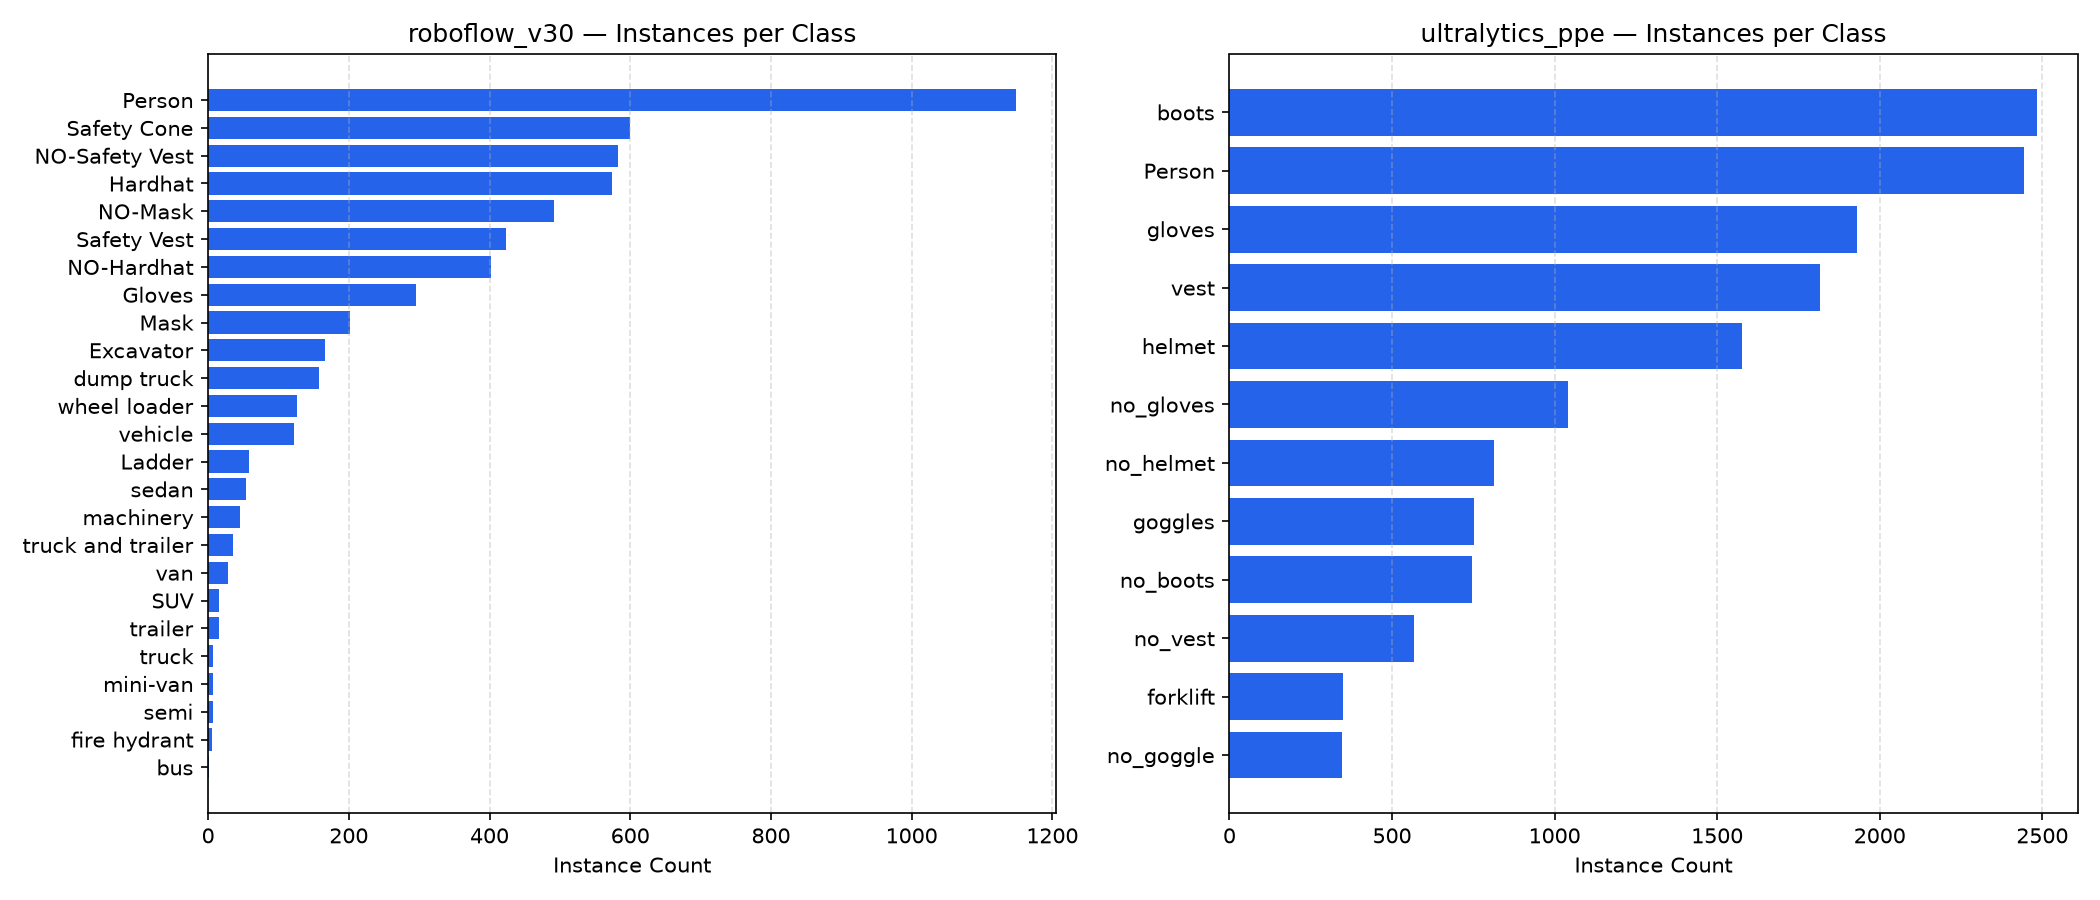
\includegraphics[width=0.92\linewidth]{reports/dataset/class_distribution.png}
  \caption{Raw class frequency distribution across Roboflow v30 and Ultralytics Construction-PPE.}
\end{figure}

\begin{figure}[H]
  \centering
  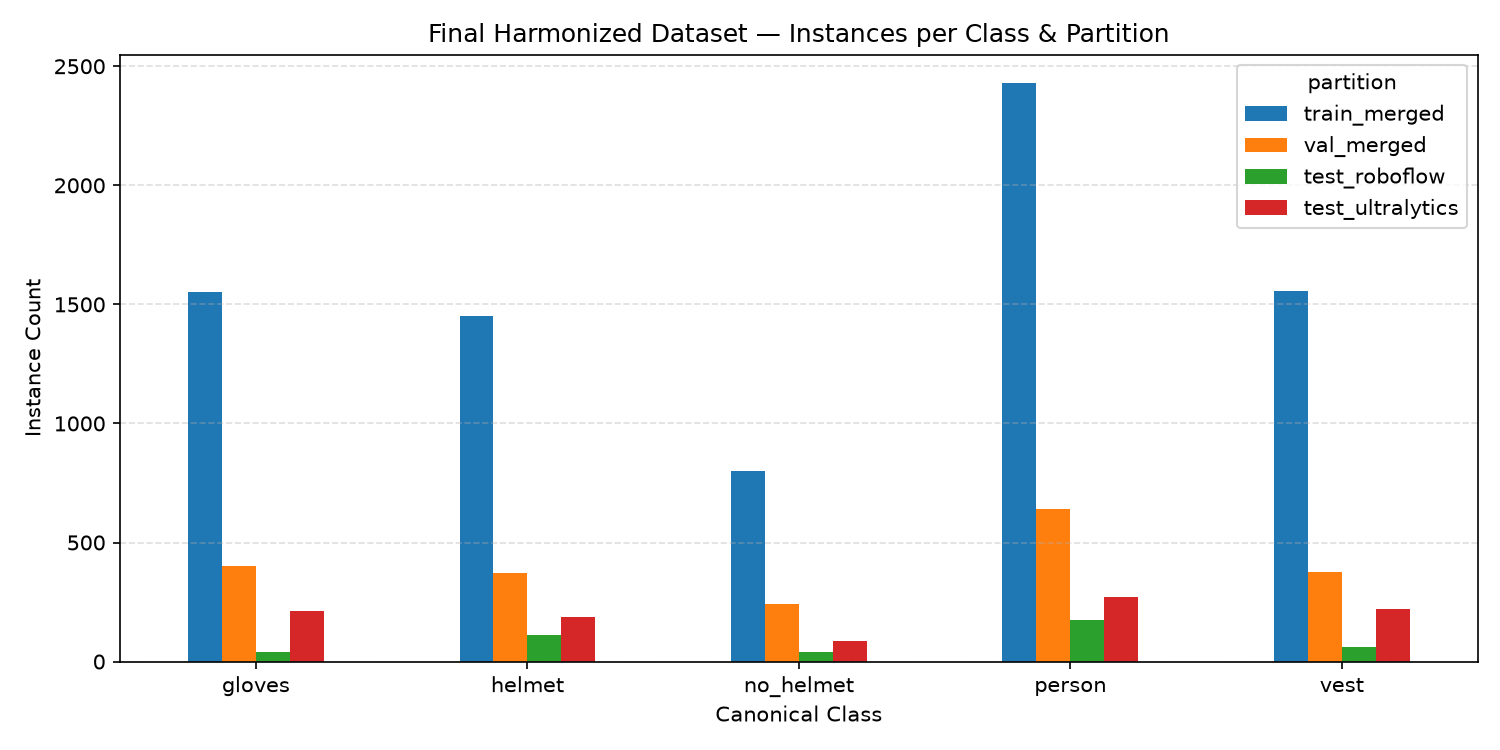
\includegraphics[width=0.92\linewidth]{reports/dataset/final_split_distribution.png}
  \caption{Final cleaned split and canonical class instance balance after leakage remediation.}
\end{figure}

\subsection{External Dataset Audit: Hard Hat Workers v10 (Rejected)}
A third public dataset (\emph{Hard Hat Workers v10}, 7,035 images, 27,039 boxes across \texttt{head}, \texttt{helmet}, \texttt{person}) was audited read-only in \texttt{docs/datasets/hard\_hat\_workers\_audit.md}. Direct integration into the 5-class detector was \textbf{rejected} for three quantitative reasons: (1) 97.03\% of images (6,826/7,035) lack \texttt{person} annotations, which would corrupt canonical \texttt{person} supervision; (2) visual inspection revealed indoor/conference crowd contamination; and (3) normalized \texttt{helmet} area is $3\times$ larger than SafeGuard's existing construction-site targets ($0.00829$ vs.\ $0.00240$--$0.00273$).

\section{Experimental Matrix, Evaluation, and Model Selection}

\subsection{Controlled Experiment Protocol}
All six experiments (\texttt{EXP-A}--\texttt{EXP-F}) trained on an NVIDIA GeForce RTX 5070 Laptop GPU at \texttt{imgsz=640}, \texttt{seed=42}, \texttt{AdamW}, tracked in MLflow (\texttt{sqlite:///mlflow.db}, experiment \texttt{SafeGuard-PPE-Detection}). \texttt{EXP-A}--\texttt{EXP-D} and \texttt{EXP-F} used 50 epochs (\texttt{lr0=0.002}), whereas \texttt{EXP-E} used 60 epochs (\texttt{lr0=0.0015}) with mild controlled augmentations (\texttt{hsv\_s=0.6}, \texttt{degrees=5.0}, \texttt{mosaic=0.8}, \texttt{mixup=0.1}).

\begin{table}[H]
\centering
\caption{Locked Test Performance Comparison Across \texttt{EXP-A}--\texttt{EXP-F} (\texttt{conf=0.25}, \texttt{iou=0.50})}
\label{tab:exp-matrix}
\small
\begin{tabular}{@{}lllrrrr@{}}
\toprule
Run & Arch & Train Scope & \multicolumn{2}{c}{\texttt{roboflow\_test} (82 imgs)} & \multicolumn{2}{c}{\texttt{ultralytics\_test} (120 imgs)} \\
\cmidrule(lr){4-5} \cmidrule(lr){6-7}
 & & & F1 & mAP@50 & F1 & mAP@50 \\
\midrule
\texttt{EXP-A} & YOLO11n & \texttt{ultralytics\_only} & 0.4669 & 0.3526 & 0.8644 & 0.8106 \\
\texttt{EXP-B} & YOLO11n & \texttt{roboflow\_only} & 0.5618 & 0.4479 & 0.5956 & 0.5032 \\
\texttt{EXP-C} & YOLO11n & \texttt{merged} & 0.6101 & 0.5089 & 0.8676 & 0.8097 \\
\texttt{EXP-D} & YOLO11s & \texttt{merged} & 0.6546 & 0.5338 & 0.8747 & 0.8211 \\
\textbf{\texttt{EXP-E}} & \textbf{YOLO11s (Tuned)} & \textbf{\texttt{merged}} & \textbf{0.6683} & \textbf{0.5610} & \textbf{0.8833} & \textbf{0.8335} \\
\texttt{EXP-F} & YOLOv8n & \texttt{merged} & 0.6254 & 0.5170 & 0.8701 & 0.8111 \\
\bottomrule
\end{tabular}
\end{table}

\subsection{Per-Class Evaluation of Selected Candidate (\texttt{EXP-E})}
Validation-only confidence sweeping (\texttt{val\_conf\_sweep.json}) confirmed optimal max-F1 behavior in $[0.25, 0.30]$, fixing deployment defaults at \texttt{conf=0.25}, \texttt{iou=0.50}. Table~\ref{tab:perclass} summarizes \texttt{EXP-E}'s per-class test metrics. Small-object false negatives dominate remaining errors: $120/152$ FN on \texttt{roboflow\_test} and $107/109$ FN on \texttt{ultralytics\_test}.

\begin{table}[H]
\centering
\caption{\texttt{EXP-E} Per-Class Detection Metrics on Both Locked Test Sets}
\label{tab:perclass}
\small
\begin{tabular}{@{}lrrrrrrrr@{}}
\toprule
Class & \multicolumn{4}{c}{\texttt{roboflow\_test}} & \multicolumn{4}{c}{\texttt{ultralytics\_test}} \\
\cmidrule(lr){2-5} \cmidrule(lr){6-9}
 & Precision & Recall & mAP@50 & mAP@50:95 & Precision & Recall & mAP@50 & mAP@50:95 \\
\midrule
\texttt{person} & 0.8112 & 0.6667 & 0.6537 & 0.4693 & 0.9669 & 0.9596 & 0.9638 & 0.8076 \\
\texttt{helmet} & 0.9625 & 0.7000 & 0.6936 & 0.4702 & 0.9214 & 0.8656 & 0.8572 & 0.6823 \\
\texttt{vest} & 0.8148 & 0.7213 & 0.6779 & 0.3943 & 0.9536 & 0.9500 & 0.9386 & 0.7667 \\
\texttt{gloves} & 0.6087 & 0.3500 & 0.3094 & 0.1823 & 0.9388 & 0.8638 & 0.8612 & 0.6663 \\
\texttt{no\_helmet} & 0.5750 & 0.5610 & 0.4706 & 0.2331 & 0.8616 & 0.5725 & 0.5467 & 0.2878 \\
\bottomrule
\end{tabular}
\end{table}

\section{ONNX Export, Numerical Parity, and Runtime Benchmarking}

The winning \texttt{EXP-E} checkpoint (\texttt{18.271 MB}) was exported to \texttt{models/production/safeguard\_yolo11s.onnx} (\texttt{36.139 MB}, ONNX opset 17, fixed input \texttt{[1,3,640,640]}, output \texttt{[1,9,8400]}) and registered in MLflow Model Registry under \texttt{SafeGuard-PPE-Detector} (Version 2, alias \texttt{@production}, run ID \texttt{8209a2eee1c4468da88f6616ab700138}).

Parity checks (\texttt{reports/benchmark/verification\_report.json}) verified:
\begin{itemize}
  \item \textbf{Class Mapping Consistency}: Exact 5-class match (\texttt{0} mismatches).
  \item \textbf{Raw Forward Tensor Parity ($N=10$)}: Max absolute error $0.00262$, mean absolute error $1.14 \times 10^{-5}$, cosine similarity $1.000$.
  \item \textbf{Same-Tensor NMS Parity ($N=10$)}: $42/42$ matched boxes ($100\%$), mean IoU $0.99989$, max coordinate error $0.005$ px.
  \item \textbf{End-to-End Pipeline Parity ($N=30$)}: $167/171$ matched ($97.66\%$), mean IoU $0.9704$, monotonic threshold sweeps.
\end{itemize}

\begin{table}[H]
\centering
\caption{Same-Hardware Runtime Benchmark Across 50 Validation Images (\texttt{benchmark\_report.json})}
\label{tab:bench}
\small
\begin{tabular}{@{}lrrrrrr@{}}
\toprule
Runtime & Size (MB) & Load (ms) & Infer Mean (ms) & E2E Mean (ms) & E2E P95 (ms) & FPS \\
\midrule
PyTorch (CPU) & 18.271 & 39.58 & 100.01 & 121.12 & 136.36 & 8.26 \\
ONNX Runtime (\texttt{CPUExecutionProvider}) & 36.139 & 96.30 & \textbf{49.70} & \textbf{67.92} & \textbf{85.86} & \textbf{14.72} \\
PyTorch (RTX 5070 Laptop GPU) & 18.271 & 265.61 & 13.75 & 38.00 & 58.55 & 26.32 \\
\bottomrule
\end{tabular}
\end{table}

\noindent On identical CPU hardware, ONNX Runtime reduces pure inference time by $2.01\times$ ($100.01\text{ ms} \rightarrow 49.70\text{ ms}$) and lowers total process peak RSS from $1076.6\text{ MB}$ to $647.0\text{ MB}$.

\begin{figure}[H]
  \centering
  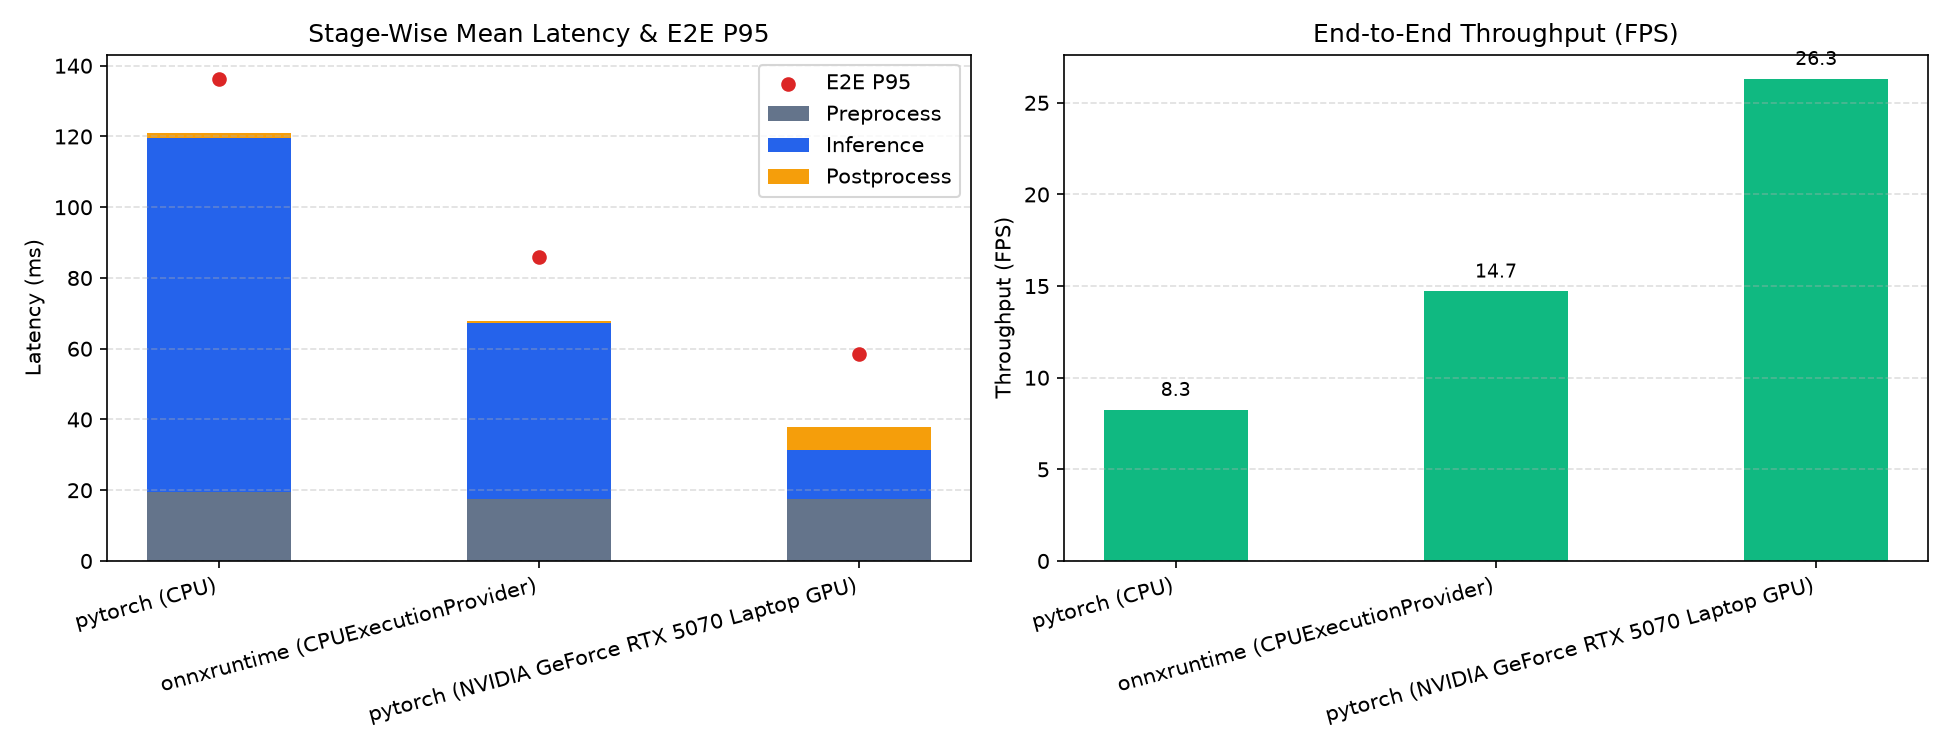
\includegraphics[width=0.90\linewidth]{reports/benchmark/latency_comparison.png}
  \caption{Latency breakdown and FPS comparison across PyTorch CPU, ONNX Runtime CPU, and PyTorch GPU.}
\end{figure}

\section{Runtime System, Anonymous Tracking, and Compliance Engine}

\subsection{FastAPI Inference Service (\texttt{backend/})}
\texttt{backend/app/main.py} loads \texttt{ONNXDetector} once during application lifespan and exposes strict Pydantic v2 contracts (\texttt{extra="forbid"}) with Swagger documentation at \texttt{/docs}, magic-byte image validation (\texttt{PIL.Image.verify}), EXIF correction, upload size/dimension caps, request-ID logging, and semantic errors (\texttt{400}, \texttt{404}, \texttt{422}, \texttt{503}, \texttt{500}):
\begin{itemize}
  \item Core inference endpoints: \texttt{GET /health}, \texttt{GET /model/metadata}, \texttt{POST /predict}, \texttt{POST /predict/visualize}, plus extensions \texttt{GET /classes} and \texttt{POST /predict/frame}.
  \item Stateful pipeline routes: \texttt{POST /predict/compliance}, \texttt{GET /compliance/alerts}, \texttt{PATCH /compliance/alerts/\{event\_id\}}, \texttt{GET /compliance/analytics}, and \texttt{POST /compliance/reset}.
\end{itemize}

\subsection{Four-Stage Tracking and Compliance Pipeline}
\begin{enumerate}
  \item \textbf{Stage 1 --- Raw Detections \& Taxonomy Validation}: Filters malformed boxes and unapproved classes against \texttt{configs/class\_mapping.yaml}.
  \item \textbf{Stage 2 --- Temporary Worker Tracking (\texttt{src/tracking/tracker.py})}: Two-stage ByteTrack IoU matcher with damped velocity prediction separating \texttt{active}, \texttt{tentative}, \texttt{lost}, and \texttt{retired} tracks without ID reuse or biometric embeddings.
  \item \textbf{Stage 3 --- Spatial Association \& Interpretation (\texttt{src/compliance/rules.py})}: Optimal 1-to-1 Hungarian matching for head (\texttt{helmet}, \texttt{no\_helmet}) and torso (\texttt{vest}) regions with multi-item matching for \texttt{gloves}. Ambiguous multi-worker overlaps fall back to \texttt{uncertain} (\texttt{ambiguous\_spatial\_overlap}); small or edge-clipped silhouettes report \texttt{insufficient\_visibility}.
  \item \textbf{Stage 4 --- Alerts \& Analytics (\texttt{alerts.py}, \texttt{analytics.py})}: Confirms explicit \texttt{no\_helmet} detections across consecutive active frames, suppresses duplicates inside cooldown windows, renders annotated JPEG evidence snapshots (\texttt{evidence\_frame\_b64}), tracks operator review status (\texttt{pending\_review}, \texttt{verified\_potential\_event}, \texttt{dismissed\_false\_alarm}, \texttt{resolved}), and aggregates stream metrics.
\end{enumerate}

\subsection{React + TypeScript Operations Console (\texttt{frontend/})}
Built with React, TypeScript (strict mode), Vite, Tailwind CSS, Recharts, and HTML5 Canvas, the UI supports three live backend-connected ingestion modes (drag/drop image upload with progress bar, 6 licensed CC BY 4.0 validation gallery samples, and bounded single-in-flight webcam monitoring with stale-frame dropping) across 8 views (\emph{Overview}, \emph{Live Monitoring}, \emph{Image Analysis}, \emph{Example Gallery}, \emph{Alert History}, \emph{Analytics}, \emph{Model Monitoring}, and \emph{Settings}), displaying separate server inference and client E2E latencies.

\section{Deployment, CI/CD, and Quality Verification}

\subsection{Containerized Multi-Service Stack}
Three isolated Docker images orchestrate via \texttt{docker compose up --build} on bridge network \texttt{safeguard\_net}:
\begin{itemize}
  \item \textbf{\texttt{backend}} (\texttt{723 MB}): Multi-stage \texttt{python:3.12-slim} non-root ONNX Runtime API mounting \texttt{./models/production:ro}.
  \item \textbf{\texttt{frontend}} (\texttt{79.9 MB}): Multi-stage Node 22 build served by \texttt{nginx:1.27-alpine} proxying \texttt{/api/} to \texttt{backend:8000}.
  \item \textbf{\texttt{mlflow}} (\texttt{1.3 GB}): Non-root MLflow server backed by named persistent volume \texttt{mlflow\_data:/mlflow}.
\end{itemize}

\subsection{Automated Verification Summary}
All code, API, browser, and container checks verified prior to publication:
\begin{itemize}
  \item \textbf{Formatting \& Linting}: \texttt{black --check .} (\texttt{33} files clean), \texttt{flake8} (0 errors), frontend \texttt{eslint .} and \texttt{tsc -b \&\& vite build} (0 errors).
  \item \textbf{Unit \& Integration Suite}: Full \texttt{pytest} suite passed (\texttt{42 passed} in training environment; \texttt{40 passed, 2 skipped} in an isolated fresh Git clone without local \texttt{.onnx} binaries).
  \item \textbf{Browser E2E}: Playwright (\texttt{tests/safeguard.spec.ts}) verified all UI pages including real Chrome webcam frames against live ONNX FastAPI with 0 console/page errors.
  \item \textbf{Docker Stack}: \texttt{docker compose up -d --build --wait} reached \texttt{Healthy} across all 3 containers; proxied \texttt{POST /api/predict} returned HTTP \texttt{200} with 12 detections.
\end{itemize}

\section{Critical Analysis and System Limitations}
\begin{enumerate}
  \item \textbf{Small-Object Recall Limits}: On wide construction views, \texttt{no\_helmet} recall remains modest ($0.5610$ RF / $0.5725$ UL), and \texttt{gloves} suffers small-object misses ($0.3500$ RF recall), leaving distant workers conservatively classified as \texttt{unknown} or \texttt{insufficient\_visibility}.
  \item \textbf{Privacy-Accuracy Trade-off in Tracking}: Pure geometric ByteTrack cannot maintain IDs across extended occlusions ($> \text{max\_age}$) or tight worker crossovers without prohibited visual/biometric Re-ID features.
  \item \textbf{Posture and 2D Projection Sensitivity}: Anatomical containment rules assume upright/semi-upright silhouettes; crouching or severe overhead angles can detach worn PPE into \texttt{unmatched\_ppe}.
  \item \textbf{Cross-Dataset \texttt{no\_helmet} Annotation Drift}: Roboflow \texttt{NO-Hardhat} often boxes only the hairline crown while Ultralytics labels the full head/face, increasing \texttt{mAP@50:95} localization variance.
  \item \textbf{MLOps Distribution Limits}: DVC currently tracks local cache/lock stages (\texttt{dvc.yaml}, \texttt{dvc.lock}); configuring an external S3/GDrive DVC remote is required before zero-copy multi-developer artifact synchronization across separate hosts.
\end{enumerate}

\section{Team Responsibilities}
\begin{itemize}
  \item \textbf{Khaled Briki (Lead Deep Learning)}: Raw dataset auditing, taxonomy harmonization, leakage deduplication, YOLO experiments \texttt{EXP-A}--\texttt{EXP-F}, ONNX parity/benchmarking, compliance rule logic.
  \item \textbf{Mohamed Amine Guesmi (Lead MLOps / DevOps)}: Git hygiene, DVC pipeline/lock maintenance, MLflow tracking \& registry deployment, Dockerfiles (\texttt{backend}, \texttt{frontend}, \texttt{mlflow}), Docker Compose networking, GitHub Actions CI workflows.
  \item \textbf{Oussama Ferchichi (Lead Full-Stack)}: FastAPI ONNX Runtime REST API, Pydantic v2 contracts, API tests, React + TypeScript console, bounded live webcam Canvas pipeline, Playwright E2E suite.
\end{itemize}

\end{document}
